\documentclass[a4paper,10pt]{article}
\usepackage[utf8x]{inputenc}
\usepackage[pdftex]{graphicx}
\usepackage{hyperref}
\usepackage{array}
\hypersetup{
    colorlinks,
    citecolor=black,
    filecolor=black,
    linkcolor=black,
    urlcolor=black
}
\hypersetup{linktocpage}


%opening
\title{Optimizations for LD-in-Couch}
\author{Teodor Macicas, eXascale, University of Fribourg - Switzerland}

\begin{document}

\maketitle
\clearpage
\clearpage

\begin{abstract}
We are going to improve the loading time of LD-in-Couch by using bulk loading/insertion or doing other low-level modifications. 
Then a comparison between the original version and optimized ones concerning the loading time, querying time and 
storage fingerprint. Also a brief discussion between optimized LD-in-Couch and CumulusRDF is provided.
\end{abstract}
\vspace{20 mm}

\section{CouchDB storage file format}
Firstly, let's have a quick look at the way CouchDB stores data on disk. This may give us a better view about what's going on.  
\paragraph{}
CouchDB stores a so-called database using only one file for both data and indexes. This may be in contrast with other databases that use different
files. Every operation is append-only and it uses copy-on-write approach. By using this it achieves no contention between multiple readers and writer. 
Thus, there is no need to use read locks. 
\paragraph{}
Another gain is that it is way faster on backup and the restore is simpler. No generation of indexes and in case the last write did not succeed a consistent state
of the file is obtained by going backward in the file (from the end) to a position where all operations had succeeded. 
This layout is also a good fit for SSD drives where the seek time is null.
\paragraph{}
However, all this advantages come also with a drawback - extra storage space. Once a document has been written, no updates will be ever done on that block. Every
update will simply create a new full document that will be appended. However, the indexes are not completely rebuilt, but a considerable space is used by this.
At the end of the newly updated document, a full branch of the indexes starting from the leaf (new document) up to the root is added. This will allow to 
get access to all other documents by exploring this branch stored at the end of the file. Actually, this is the ``header`` of the file. 
\paragraph{}
An workload implying milions of documents with many updates will create huge files. A compaction is then required to shrink the space used.
\paragraph{}
For further detailed information please have a look here: \newline\url{https://github.com/couchbaselabs/couchstore/wiki/Format} 
\newline\url{https://plus.google.com/u/0/107397941677313236670/posts/CyvwRcvh4vv}

\section{Bulk load in CouchDB}
LD-in-Couch Python script has been modified to allow bulk insertion. A parameter defines how many documents should be collected before an insertion is done. 
After testing with 1k, 5k, 10k, 50k as the granularity parameter while inserting, 10k has proved to be the best / fastest option for our installation. 
\paragraph{}
On the following sections we present two different versions of optimized LD-in-Couch. The first one is simpler, but faster by dropping some features. 
The second one enabled the dropped features by employing a longer loading time. 

\subsection{First approach - one document per each triple}
This first approach of optimizing LD-in-Couch is simply creating a document for each (s,p,o) triple read from the input file. Thus, many different documents
with same subject value can coexit. 
\paragraph{}
However, the back-links feature are totally discarded for this approach. The unoptimized version used a ''by\textunderscore subject`` view for querying 
the already loaded database for a document having as subject the current object value. Obviously, this process is very slow as for each document that 
needs to be loaded a lookup on disk is required. 
\paragraph{}
In order to offer querying by subject feature, a view must be created after the whole input file is loaded. This step takes also time and it is expected to 
be roughly the same as the initial loading time (as a view is actually a materialized view over all the DB). The total time is shown Table~\ref{tab:loading_times} 
in between parantheses. As a bottom line, this approach is way faster than the initial version, but the tradeoff was to drop some features (i.e. efficient structure, 
back-links, querying by object).

\subsection{Second approach - one document per each subject}
Having one document for each triple would imply having multiple documents for each subject which may not be efficient. Thus, this second approach of optimizing 
LD-in-Couch aims to group all predicates and objects belonging to the same subject within one single document (just as the unoptimized version does).\newline
In order to do this, we now keep a hashset of all already loaded subjects and whenever a new line is read it is checked if an update is needed or a 
new document must be created. The hashset ensures that a disk operation is worth (i.e. by the time disk is accessed we are sure there is a document). \newline 
Because we are using bulk-load, we firstly look whether or not a document with same subject exist in the not-yet-loaded cache. This speeds up compared to going 
to disk every time. 
\paragraph{}
One good observation is that instead of assigning random hexa-decimal IDs to every document, we could re-\textit{use the subject as an ID}, as it is unique.
By doing this, we don't need anymore another view for querying ''by\textunderscore subject`` - but querying by ID using the subject itself does the job. \newline
However, we still lack the back-links. We experimented by including them on the loading process, but it proved to take too much time (i.e. 3 hours for 1mil dataset). 
To overcome this, we propose to use a ''by\textunderscore object`` view by paying the extra cost of space and time. This will create a mapping (key, value) between 
an object and a predicate. The subject is not needed as part of 'value' because it is stored as ''id``. Thus, many mappings having the same subject value will
be created. We tried to compress this into only one by using the ''reduce`` function whilst view creating, but it proved to be too slow.
Therefore, just a simple map function is provided. \newline 
Compared to previous versions, another ''by\textunderscore predicate`` view is created. This maps a prediate to an object and, as explained above, it also creates 
one document for each mapping. This is way faster than using ''reduce`` functions. Having this, we can also query by predicate. \newline 
We realized that the space of the views is considerable higher than the DB itself, thus a compaction is needed and it proved to save space. Therefore the following
actions are undertaken here: 
\begin{itemize}
 \item loading triples using a caching mechanism + bulk loading 
 \item creating the by\textunderscore subject and by\textunderscore object views
 \item compaction of the just created views (running as background job and the old view is readable)
\end{itemize}

\subsection{Datasets}
\paragraph{}
All the datasets used for testing were previously sorted by subject. By using such a .nt file we get better performance as there are fewer
disk accesses for updating an already loaded document. Mostly of the updates are done in the cache in case of bulk loading.
\paragraph{}
First datase was given by the university administrator. It contains information about teaching units, professors, departments and fields of studies. 
Let's call it \textit{Faculty dataset}. 
\paragraph{}
Besides the Faculty datasets, we also experimented with two others - \textit{Bowlogna} and \textit{Linkedmdb}. The former is generated by with the help
of the BowlognaBench generator. The latter is taken from DBpedia and contains information about movies and actors. It is relatively 
equally distributed in terms of number of triples per entity. 

\begin{table}[h]
\centering
\begin{tabular}{|>{\centering}p{2cm}|>{\centering}p{2cm}|>{\centering}p{2cm}|>{\centering}p{2cm}|>{\centering}p{2cm}|}
    \hline 
    dataset & \# triples & \#uniq subj & \#uniq pred & \#uniq obj \tabularnewline
    \hline
    \hline 
    Faculty & 10,693 & 1,745 & 35 & 1,403 \tabularnewline
    \hline 
    Faculty & 97,336 & 15,496 & 35 & 9,193 \tabularnewline
    \hline 
    Faculty & 704,882 & 111,847 & 35 & 65,899 \tabularnewline
    \hline
    Faculty & 4,816,009 & 764,205 & 35 & 433,248 \tabularnewline
    \hline
    Bowlogna & 1,236,465 & 213,037 & 39 & 26,300 \tabularnewline
    \hline
    \multicolumn{2}{l}{Avg entities per subject:} 6.15 \\
    \cline{1-2}
    \hline
    Linkedmdb & 6,148,121 & 694,400 & 223  & 1,503,645 \tabularnewline
    \hline
    \multicolumn{2}{l}{Avg entities per subject:} 8.85 \\
    \cline{1-2}
\end{tabular}
\caption{Unique subj/pred/obj for all datasets}
\label{tab:uniq_data_sets}
\end{table}

\subsection{Loading time}
Let's have a look how the loading time has changed under different datasets. Since way fewer, but larger documents are created for the 2nd optimized version, the 
loading time is slightly lower. Do not forget, that 2nd version creates two views (object + predicate) rather than just one (object). 

\begin{table}[h]
\centering
\begin{tabular}{|>{\centering}p{1.5cm}|>{\centering}p{1.8cm}|>{\centering}p{2cm}|>{\centering}p{2.5cm}|>{\centering}p{2.5cm}|}
    \hline 
    dataset name & \# triples & LD-in-Couch & optimized 1st (+view creation) & optimized 2nd (+views creation) \tabularnewline
    \hline
    \hline 
    Faculty & 10,693 & 26m15s & 0m2s (0m5s) & 0m1s (0m2s) \tabularnewline
    \hline 
    Faculty & 97,336 & 4h18m13s & 0m16s (0m30s) &  0m6s (0m15s) \tabularnewline
    \hline 
    Faculty & 704,882 & 2d32h41m & 1m46s (3m06s) & 0m50s (2m43s) \tabularnewline
    \hline
    Faculty & 4,816,009 & N/A & 12m44 (25m10s) & 5m55s (20m47s) \tabularnewline
    \hline
    \hline
    Bowlogna & 1,236,465 & N/A & N/A & 1m31s (5m54s) \tabularnewline
    \hline
    Linkedmdb (DBpedia) & 6,148,121 & N/A & N/A & 7m3s (16m27s) \tabularnewline
    \hline
\end{tabular}
\caption{Optimized LD-in-Couch loading times of all datasets}
\label{tab:loading_times}
\end{table}

\paragraph{}
Table~\ref{tab:data_sizes} shows how much physical space is needed for different versions and data sets. The storage space has been measured by directly 
looking on the data directory configured at installation time. For each data set, there are two numbers - first represents the size needed by only the data and 
the second comprises also views compacted sizes. 

\begin{table}[h]
\centering
\begin{tabular}{|>{\centering}p{1.5cm}|>{\centering}p{1.5cm}|>{\centering}p{1.8cm}|>{\centering}p{2cm}|>{\centering}p{2cm}|>{\centering}p{2cm}|}
    \hline 
    dataset name & \# triples & LD-in-Couch & Compacted LD-in-Couch & optimized 1st (+view creation) & optimized 2nd (+views creation) \tabularnewline
    \hline
    \hline
    \hline 
    Faculty & 10,693 & 98MB (154MB) & 1.4MB (3.2MB) & 3,2MB (6.7MB) & 0.9MB (1.9MB) \tabularnewline
    \hline 
    Faculty & 97,336 & 1.9GB (2.9GB) & 15MB (21.8MB) & 29MB (55.2MB) & 8.2MB (16.9MB) \tabularnewline
    \hline 
    Faculty & 704,882 & 44GB (76GB) & 116MB (327MB) & 220MB (0.5GB) & 65MB (126MB) \tabularnewline
    \hline
    Faculty & 4,816,009 & N/A & N/A & 1.5GB (4.1GB) & 557MB (993MB) \tabularnewline
    \hline
    \hline
    Bowlogna & 1,236,465 & N/A & N/A & N/A & 155MB (326MB) \tabularnewline
    \hline
    Linkedmdb & 6,148,121 & N/A & N/A & N/A & 399MB (887MB) \tabularnewline
    \hline
\end{tabular}
\caption{Optimized LD-in-Couch storage space used by Faculty datasets}
\label{tab:data_sizes}
\end{table}

\paragraph{}
As expected, the 2nd version is more efficient on using data storage because it compresses multiple predicates and objects belonging to the same subject. 
Also it looks like bulk loading uses also better the disk space if we compare the footprint with the compacted verison. \newline 
Since the views have been compacted their size is way smaller even though there are two instead of one as we had on the first optimized version.

\subsection{Loading time - optimized LD-in-Couch vs CumulusRDF}
Let's see a one to one comparison with CumulusRDF (Cassandra based - for futher information please refer to 
''ld\textunderscore in\textunderscore couch-vs-cumulus\textunderscore rdf.pdf`` page 7). \newline
As it was already seen (the other document), the query time is roughly the same, so here we just focus on comparing the loading times.
\paragraph{}
Be aware that y axis of the figure~\ref{fig:loading_time_comparison} is logarithmic. 
Cassandra's bulk-load feature can be one magnitude of order faster than the CouchDB's version. 
\begin{figure}[h!]
  \centering
  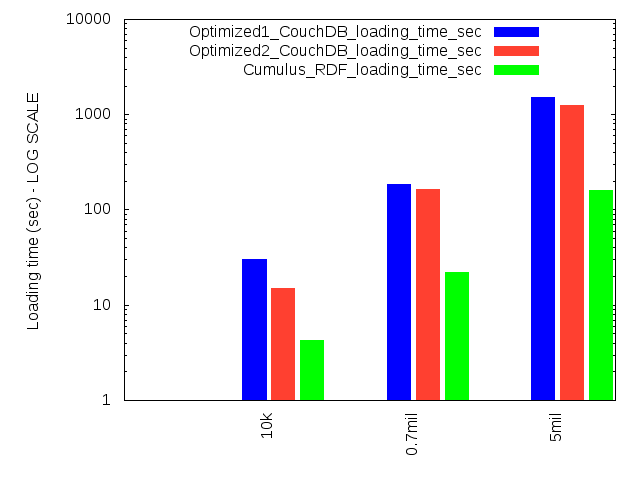
\includegraphics[height=200px]{../optimized_couchdb/loading_time.png}
  \caption{Optimized LD-in-Couch vs CumulusRDF loading time}
  \label{fig:loading_time_comparison}
\end{figure}

\section{Querying time}
Here we give a short overview how the querying time has been affected by using the optimized versions. 
We assume that the required views have been already created before a query is fired. Otherwise, the execution time of 
the first query will take considerable long time as the view is lazily updated / created. 
\paragraph{}
Overall, the querying times of the optimized versions are comparable with those of the compacted versions. Therefore, please refer to the document 
''ld\textunderscore in\textunderscore couch-vs-cumulus\textunderscore rdf.pdf`` page 7 to get more information.



\paragraph{}
Following tables show the execution times for different random queries using four different datasets.
\begin{table}[h]
\centering
\begin{tabular}{|>{\centering}p{2.5cm}|>{\centering}p{2.5cm}|>{\centering}p{2.5cm}|>{\centering}p{2.5cm}|}
    \hline 
    dataset name & \# triples & 100 queries & 1000 queries \tabularnewline
    \hline
    \hline 
    Faculty & 10,693 & 1.1s & 10.44s \tabularnewline
    \hline 
    Faculty & 97,336 & 1.1s & 10.7s \tabularnewline
    \hline 
    Faculty & 704,882 & 1.0s & 10.7s \tabularnewline
    \hline
    Faculty & 4,816,009 & 2.0s & 24.06s \tabularnewline
    \hline
    \hline
    Bowlogna & 1,236,465 & 1.86s & 22.409s \tabularnewline
    \hline
    Linkedmdb & 6,148,121 & 3.867s & 29.912s \tabularnewline
    \hline
\end{tabular}
\caption{By subject (as id) querying times}
\label{tab:query_times_subj}
\end{table}

\begin{table}[h]
\centering
\begin{tabular}{|>{\centering}p{2.5cm}|>{\centering}p{2.5cm}|>{\centering}p{2.5cm}|>{\centering}p{2.5cm}|}
    \hline 
    dataset name & \# triples & 100 queries (\#results) & 1000 queries (\#results)  \tabularnewline
    \hline
    \hline 
    Faculty & 10,693 & 2.031s (21,568) & 20.46s (214,175) \tabularnewline
    \hline 
    Faculty & 97,336 & 5.57s (162,412) & 63.7s (2,127,017) \tabularnewline
    \hline 
    Faculty & 704,882 & 51.356s (2,432,918) & 450.373s (21,118,534) \tabularnewline
    \hline
    Faculty & 4,816,009 & 246.742s (12,059,250) & /too long/ \tabularnewline
    \hline
    \hline
    Bowlogna & 1,236,465 & 110.66s (4,802,190) & /too long/ \tabularnewline
    \hline
    Linkedmdb & 6,148,121 & 59.385s (2,865,816) & 670.063s (32,222,407) \tabularnewline
    \hline
\end{tabular}
\caption{By object (as view) querying times}
\label{tab:query_times_obj}
\end{table}

\begin{table}[h]
\centering
\begin{tabular}{|>{\centering}p{2cm}|>{\centering}p{2cm}|>{\centering}p{2cm}|>{\centering}p{2cm}|>{\centering}p{2cm}|}
    \hline 
    dataset name & \# triples & 10 queries (\#results) & 100 queries (\#results) & 1000 queries (\#results)  \tabularnewline
    \hline
    \hline 
    Faculty & 10,693 & 0.487s (10,391) & 4.298s (95,878) & 43.957s (968,325) \tabularnewline
    \hline 
    Faculty & 97,336 & 2.629s (112,656) & 24.437s (1,045,699) & 234.487s (10,016,472) \tabularnewline
    \hline 
    Faculty & 704,882 & 24.727s (1,152,568) & 216.646s (10,250,715) & /too long/ \tabularnewline
    \hline
    Faculty & 4,816,009 & 103.886s (4,971,825) & /too long/ & /too long/ \tabularnewline
    \hline
    \hline
    Bowlogna & 1,236,465 & 46.098s (1,962,127) & 431.34s (18,435,419) & /too long/ \tabularnewline
    \hline
    Linkedmdb & 6,148,121 & 37.629s (1,992,655) & 647.981s (33,103,746) / & /too long/ \tabularnewline
    \hline
\end{tabular}
\caption{By predicate (as view) querying times}
\label{tab:query_times_pred}
\end{table}

\subsection{Example of queries}
\subsubsection{By subject}
\paragraph{Non-optimized version}
\paragraph{}
Querying the by\textunderscore subject view:
\begin{verbatim}
curl -X GET 
'http://localhost:5984/replicate_rdf1mil/_design/entity/_view/by_subject?
key="http%3A//www.owl-ontologies.com/Ontology1347094758.owlrepo1mil_test"'
\end{verbatim}
)
Query result is a key,value tuple. The value is actually the document itself. By taking values from o\textunderscore in parameter 
we can explore further the RDF graph.
\begin{verbatim}
{"id":"1016b8034c1dc728e6d1826bb052feb2",
 "key":"http://www.owl-ontologies.com/Ontology1347094758.owlrepo1mil_test",
 "value":
    {"_id":"1016b8034c1dc728e6d1826bb052feb2",
     "_rev":"1-93df73c494ff8e2a96b2806b4df744e9",
     "doc_type":"RDFEntity","g":"repo1mil_test",
     "s":"http://www.owl-ontologies.com/Ontology1347094758.owl",
     "p":["http://www.w3.org/1999/02/22-rdf-syntax-ns#type"],
     "o_in":[],"o":["http://www.w3.org/2002/07/owl#Ontology"]}}
}
\end{verbatim}

\paragraph{Optimized 1st version}
\paragraph{}
Please check the non-optimized version. The difference is that we don't get the o\textunderscore in parameter, so we cannot explore further. 

\paragraph{Optimized 2nd version}
\paragraph{}
As the subject is acutally the document ID, we just have to query by ID using the subject. Pay attention to escaping special chars !
\begin{verbatim}
curl -X GET 'http://localhost:5984/optimized2_1mil/
http%3A%2F%2Fwww.owl-ontologies.com%2FOntology1347094758.owl'
\end{verbatim}

The result is exactly the document and now we can take the object value and query by object to explore further.
\begin{verbatim}
 {"_id":"http://www.owl-ontologies.com/Ontology1347094758.owl",
  "_rev":"1-1b27c88b1f4ba16e6fd2255b9006259a",
  "doc_type":"RDFEntity","g":"optimized2_1mil",
  "o":["http://www.w3.org/2002/07/owl#Ontology"],
  "p":["http://www.w3.org/1999/02/22-rdf-syntax-ns#type"],
  "s":"http://www.owl-ontologies.com/Ontology1347094758.owl"}
\end{verbatim}


\subsubsection{By object}
\paragraph{Non-optimized version}
\paragraph{}
By using the values in ''o\textunderscore in`` we can query once again by subject and get the documents we are interested in.


\paragraph{Optimized 1st version}
\paragraph{}
This version does not offer a query mechanism by object. However, it can still be done if a ''by\textunderscore object`` view is created (as it 
has been done for the 2nd version - however this would increase the footprint).


\paragraph{Optimized 2nd version}
\paragraph{}
In this case after querying by subject, we just get the object and fire a query ''by\textunderscore object``. The query looks like: 

\begin{verbatim}
curl -X GET 'http://localhost:5984/optimized2_1mil/_design/entity/_view/
by_object?key="http%3A//www.w3.org/2002/07/owl%23Ontology"'
\end{verbatim}

As expected the result is a key,value tuple. The key is the object about which we queried. The value contains just the predicate as the subject is 
reflected by ''id`` (as we did not use hexa-decimal random IDs, but the subject). Therefore, querying by ID would return the full document if needed. 
\begin{verbatim}
{"id":"http://www.owl-ontologies.com/Ontology1347094758.owl",
 "key":"http://www.w3.org/2002/07/owl#Ontology",
 "value":
    {"p":"http://www.w3.org/1999/02/22-rdf-syntax-ns#type"}
}
\end{verbatim}

\subsubsection{By predicate}
\paragraph{Non-optimized version}
\paragraph{}
This version contains no by\textunderscore predicate view. 

\paragraph{Optimized 1st version}
\paragraph{}
This version contains no by\textunderscore predicate view. 

\paragraph{Optimized 2nd version}
\paragraph{}
In this case after querying by subject, we just get the predicate and fire a query ''by\textunderscore predicate``. The query looks like: 

\begin{verbatim}
curl -X GET 'http://localhost:5984/optimized2_1mil/_design/entity/_view/
by_predicate?key="http%3A//www.unifr.ch/philosophy.owl%23beginsOnDate"'
\end{verbatim}

As expected the result is a key,value tuple. The key is the predicate about which we queried. The value contains just the object as the subject is 
reflected by ''id`` (as we did not use hexa-decimal random IDs, but the subject). Therefore, querying by ID would return the full document if needed. 
\begin{verbatim}
{"id":"http://www.unifr.ch/philosophy.owl#Semester0",
 "key":"http://www.unifr.ch/philosophy.owl#beginsOnDate",
 "value":{"o":"2005-09-19\"^^<http://www.w3.org/2001/XMLSchema#string"}
},
[ ... ]
\end{verbatim}

\section{Conclusion}
CouchDB way of storing documents is suitable for SSD drives and offers a fast recovery in case of failures due to its append-only mechanism. Also the 
indexes are stored on the same file, just after the document itself. By doing this, one can get access to whichever document just by reading the 
so-called ''file header`` placed at the end. However, the tradeoff comes on the disk space. 
\paragraph{}
By using the bulk-loading feature of CouchDB we managed to make way faster the insertion of RDF triples on LD-in-Couch. We simply modified the Python script and 
there is no more one-single-record-insertion but bulk. As experimented, 10.000 records to insert once has proved to be the fastest on our system. 
\paragraph{}
Bulk-loading enforces a change of the database schema. On the unoptimized version one document is created for each unique subject (used as key) and inside it an array 
of pairs (predicate,object) is stored. Also a field named ''o\textunderscore in`` stored all back-links of that subject. The structure is slightly different. \newline
The first optimized version dropped this compressed structure and creates a document per each triple read from the input file. Also the back-links were dropped 
for the sake of a better performance. However, for our use case this is not suitable and the storage space is not efficiently. Therefore, a second optimized 
version has been develoed. \newline. 
By using a cache mechanism and enforcing to use the subject as a document ID (not a hexa-decimal random value), we were able to faster bulk-load, but still keeping the 
one document per unique subject structure. Nevertheless, creating the ''o\textunderscore in`` parameter would still take too much time. An workaround for this is to 
create a ''by\textunderscore object`` view. Aslo a ''by\textunderscore predicate`` view is created to enable querying by predicate. For saving storage space, a 
compaction of all views is done as a background job.
\paragraph{}
The outcome has an acceptable performance concerning the loading times (see table~\ref{tab:loading_times} and figure~\ref{fig:loading_time_comparison}), 
but still one order of magnitude slower than Cassandra. On the other side, the query time remains comparable with CumulusRDF as well as with the 
compacted versions of LD-in-Couch. 

\clearpage
\end{document}